\documentclass{report}
\usepackage{graphicx} % Required for inserting images
\usepackage{tcolorbox}
\usepackage{amsfonts}
\usepackage{amsmath}
\usepackage{parskip}
\usepackage{hyperref}

\bibliographystyle{plain} % We choose the "plain" reference style
\graphicspath{ {./images/} }

\title{Statistical Neuroimaging}
\author{Joel Winterton}
\date{November 2023}

\begin{document}
\maketitle
\tableofcontents

\chapter{Segmentation via Weighted Aggregation}

\section{Objective - Why we want to do this}
The objective of using the method of Segmentation via Weighted Aggregation in this context, is to extract a range of features from each aggregate, and then train a random forest on all of the features we obtain (from multiple images), after feature extraction, the classifier is agnostic to the image. 

So we are training our random forest on a dataset 
\[\mathbf{f} = \{f_1, ... , f_m\}\]
where each $f_i$ is a vector of features extracted on an aggregate indexed as aggregate $i$.

Any complication that arise from interpolation e.t.c. arise because we are aiming to keep linear time complexity. 

\textcolor{red}{Could try exploring a more intuitive, less efficient segmentation algorithm first?}

\section{Overview - How we're going to do it}
This is a more in detail version of \cite{sharon_galun_sharon_basri_brandt_2006}.
\begin{enumerate}

\item Make a graph of the image $G^{(1)}$, each pixel is a node and edges are between neighbouring pixels. 
\item Edge weights are called an affinity, lower affinity means pixels are more "different" in some sense.
\item Aim to construct a new graph which is a coarsening of the old one, by first choosing which nodes in the graph to keep (the seeds).
\item Then decide how to interpolate the values of the non-seeds (values being for instance intensity) into the new seeds.
\item Determine what the edge weights of the new coarse graph is. 
\item Calculate and store the features of each node in the new coarse graph, these new nodes are also referred to as "aggregates". 
\item Repeat this coarsening process. 
\end{enumerate}
\section{Nitty Gritty}
\subsection{Graph Initialisation}
\textbf{Covering steps 1 and 2.}
Let $G(V, E)$ be a graph where each vertex is a pixel in the image. In implementation it is easiest to do this by denoting each node by it's position in the image with a "nice" origin (a top corner for instance). Two nodes are adjacent in this graph if they are neighbours (horizontally, vertically or diagonally) in the image.
 
Then for any edge $(u,v)\in E$ define the weight function as an affinity: 
\[w_{uv} = \exp{(-d(u,v; \alpha))}\]
where $d$ is some distance metric of the nodes. \cite{galun_sharon_basri_brandt_2003} uses the Euclidean distance of intensities of the pixels as the distance metric: 
\[d(u,v) = \alpha|I_u - I_v|_2\]

This graph doesn't have to represent a singular image, and this distance metric can be used to include multiple images (referred to as multi-channel) \cite{akselrod-ballin_galun_gomori_filippi_valsasina_basri_brandt_2009}. This is useful as MR scans can have several channels (T-1, T-2 and FLAIR being the common channels). 

The next few steps only require the previous graph, so assume that we have a graph $G^{(i-1)}(V^{(i-1)}, E^{(i-1)})$, where $n^{(i-1)} = |V^{(i-1)}|$, and we are aiming to construct a coarser graph $G^{(i)}(V^{(i)}, E^{(i)})$.

\subsection{Seed selection}

\textbf{Covering step 3-5}
The idea here is to group up nodes of the previous graph in a way that maintains some sort of strong coupling between the nodes being merged together, this group of nodes will be referred to as a segment. This can be thought of in terms of graph cuts. We are aiming to find cuts of a graph that maximise some similarity between nodes inside cliques, while keeping the difference between nodes adjacent across a cut high. For any segment $S \subset V^{(i-1)}$ let $\mathbf{u} = (u_1, ..., u_{n^{(i-1)}})$ denote the segment, where 
\begin{equation*}
u_i = \begin{cases} 1 & \text{if}\: \: v_i \in S \\
0 & \text{else}
\end{cases}
\end{equation*}
We sum the weights of all the edges on the boundary of the segment using the fact that $(u_i - u_j)^2 = 1$ if nodes are on the boundary of the segment, and everywhere else $(u_i - u_j)^2 = 0$ everywhere else. Hence the sum of weights on the boundary is given by: 
\[
\sum_{i>j} w_{ij}(u_i - u_j)^2
\]

We then sum over all edge weights inside segment,  using that $u_iu_j = 1$ if both nodes are in segment and $u_iu_j=0$ otherwise. Hence the "weight volume" is given by: 
\[\sum_{i>j} w_{ij}u_iu_j\]

We can then define the so-called saliency of a segment $\Gamma(\mathbf{u})$, which is the sum of all boundary weights normalised by the weight volume: 
\[\Gamma(\mathbf{u}) = \frac{\sum_{i>j} w_{ij}(u_i - u_j)^2}{\sum_{i>j} w_{ij}u_iu_j}\]
 
This can be expressed more compactly using the Graph Laplacian matrix $L$ with entries
\[L_{ij} = 
\begin{cases}
\sum_{k: k \neq i} w_{ik} & \text{if} \: \: i=j \\
w_{ij} & \text{else}
\end{cases}\]
along with the weight matrix $W$ with entries
\[W_{ij} =\begin{cases}
w_{ij} & \text{if} \: \: (v_i, v_j) \in E \\
0 & \text{else}
\end{cases} \]
Hence 
\[\Gamma(\mathbf{u}) = \frac{\mathbf{u}^TL\mathbf{u}}{\frac{1}{2}\mathbf{u}^TW\mathbf{u}}\]
\begin{figure}[h]
\centering
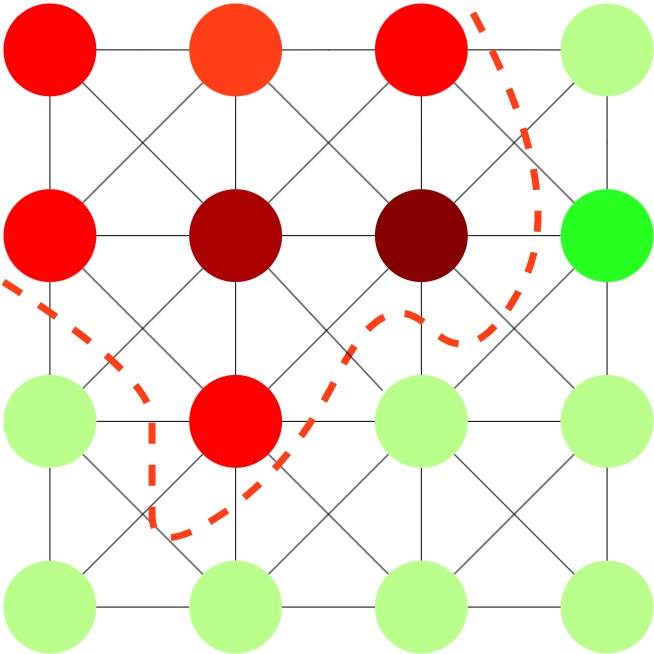
\includegraphics[width=0.3\textwidth]{GraphCutExample}
\caption{Example of a graph cut with high saliency.}
\end{figure}


To do this, a measure is defined that takes into account the contrast over the boundary of a segment, as well as the similarity of the 












\chapter{Introduction}
The current general aim of the project is to explore and implement methods that identify brain lesions from an MRI scan.  The dataset that we have is 36 people, and several other datasets are similarly sized. 

\section{Random Forests}
The primary method to be explored is using Random Forests.
\begin{itemize}
	\item There will need to be significant changes to learning process so as to be applicable to 2D images (or indeed 3D images). 
	\item Another complication is that the images are anisotropic, and so either pre-processing correction is needed, or the learning process will need to take this into account.
\end{itemize}
\chapter{Rough notes}
\section{General resources}
\subsection{General Imaging and MRI Pipeline}
Need to construct a general overview medical imaging, maybe going into slightly more detail about MRI scan pipeline. 
\subsection{MS Lesion Segmentation Pipeline}
For MS lesion segmentation pipeline, can use elpful overview from \href{https://pdf.sciencedirectassets.com/271303/1-s2.0-S0895611118X00081/1-s2.0-S0895611118303227/main.pdf}{Survey of automated multiple sclerosis lesion segmentation
techniques on magnetic resonance imaging}
\section{Isolated Concepts}
\subsection{Random Forests}
Need to understand what "Random forests require heirarchy" means and how this can be applied to images (what does it mean to extract heirarchy from an image)
\subsection{Segmentation and Heirarchy}
Explore Segmentation by Weighted Aggregation method. Explore how heirarchy is obtained from an image.
\section{Scale Space / Smoothing}
Scale space seems to be deeply connected to the smoothing of an image using a Gaussian Kernel. 
\textbf{\textcolor{red}{Todo}}
\begin{itemize}
\item Explore and understand image scale space, along with the motivating idea behind segmentation. 
\item Explore scale space segmentation \href{https://en.wikipedia.org/wiki/Scale-space_segmentation}{Wikipedia page}.
\item Explore Segmentation by Weighted Aggregation method.
\end{itemize}

\section{Todo}
Then reattempt to understand some of \href{https://ieeexplore.ieee.org/stamp/stamp.jsp?tp=&arnumber=5238795}{Automatic Segmentation and Classification
of Multiple Sclerosis in Multichannel MRI}. The main heuristic of this paper is to do MS lesion segmentation in MRI scans by training Random Forests at a multiscale level. Then explore the more advanced version of this: Spatially Adaptive Random Forests \href{https://ieeexplore.ieee.org/document/6556781}{Spatially Adaptive Random Forests
}.

\chapter{Question}
\bibliography{references}

\end{document}
